\part{Introduksjon til Optimering}
\label{part:introduction}

\chapter{Teori}
\label{chap:mathematical_foundations}

\section{Lineær Algebra}

\subsection{Vektor-- og matriseoperasjoner}

\subsubsection{Indre produkt}
Det indre produktet, også kjent som skalarprodukt, er en operasjon som tar to vektorer og gir et tall.
Dette tallet representerer på mange måter hvordan vektorene "overlapper" med hverandre, og er spesielt nyttig for å måle avstander og vinkler mellom vektorer.

\begin{definition}{Indre produkt}{inner_product}
	Gitt to vektorer \( \symbf{u}, \symbf{v} \in \R^n \), er det indre produktet definert som:
	\[
		\symbf{u} \cdot \symbf{v} = \symbf{u}^\top \symbf{v} = \sum_{i=1}^{n} u_i v_i
	\]
\end{definition}

\begin{corollary}{Vektorprojektering}{vector_projection}
	Projeksjonen av vektoren \( \symbf{u} \) på vektoren \( \symbf{v} \) er gitt ved:
	\[
		\operatorname{proj}_{\symbf{v}}(\symbf{u}) = \frac{\symbf{u} \cdot \symbf{v}}{\norm{\symbf{v}}^2} \symbf{v}
	\]
	Dette gir oss en ny vektor som er parallell med \( \symbf{v} \) og representerer den delen av \( \symbf{u} \) som "går i retning" av \( \symbf{v} \).
\end{corollary}

\subsubsection{Ytre produkt}
Ytre produktet er en operasjon som tar to vektorer og lager en matrise.
\begin{definition}{Ytre produkt}{outer_product}
	Gitt to vektorer \( \symbf{u} \in \R^m \) og \( \symbf{v} \in \R^n \), er det ytre produktet definert som:
	\[
		\symbf{u} \otimes \symbf{v} = \symbf{u} \; \symbf{v}^\top =
		\begin{bmatrix}
			u_1v_1 & u_1v_2 & \cdots & u_1v_n \\
			u_2v_1 & u_2v_2 & \cdots & u_2v_n \\
			\vdots & \vdots & \ddots & \vdots \\
			u_mv_1 & u_mv_2 & \cdots & u_mv_n
		\end{bmatrix}
	\]
\end{definition}

\subsubsection{Norm}
En norm er en funksjon som måler \enquote{størrelsen} eller \enquote{lengden} av matematiske objekter som vektorer.
Den generaliserer ideen om absolutt verdi til høyere dimensjoner.

\begin{definition}{Norm}{norm}
	En norm på et vektorrom \(V\) er en funksjon \(\norm{\cdot}: V \to \R\) som oppfyller:
	\begin{enumerate}
		\item \textbf{Positivitet:} \(\norm{\symbf{x}} \geq 0\) og \(\norm{\symbf{x}} = 0\) hvis og bare hvis \(\symbf{x} = 0\)
		\item \textbf{Homogenitet:} \(\norm{\alpha \symbf{x}} = |\alpha| \norm{\symbf{x}}\) for alle \(\alpha \in \R\)
		\item \textbf{Trekantulikhet:} \(\norm{\symbf{x} + \symbf{y}} \leq \norm{\symbf{x}} + \norm{\symbf{y}}\)
	\end{enumerate}
\end{definition}

\begin{remark}{Viktige normer}{important_norms}
	De mest brukte normene i \(\R^n\) er:
	\begin{align*}
		\tag{Euklidisk norm} \norm{\symbf{x}}_2 & = \sqrt{\sum_{i=1}^{n} x_i^2} \\
		\tag{Manhattan norm} \norm{\symbf{x}}_1 & = \sum_{i=1}^{n} |x_i|        \\
		\tag{Max norm} \norm{\symbf{x}}_\infty  & = \max_{i=1,\ldots,n} |x_i|
	\end{align*}
	Den euklidiske normen er den mest vanlige og svarer til vår intuitive forståelse av avstand.
\end{remark}

\section{Mengder}

\subsection{Baller}
En ball i \(\R^d\) er en mengde av punkter som ligger innenfor en viss avstand fra et sentrumspunkt. Den kan være åpen eller lukket, avhengig av om grensen er inkludert eller ikke.
Den er definert ved den euklidiske normen\eqref{eq:euclidean_norm}.

\paragraph{Åpen Ball}
En åpen ball i \(\R^d\) er mengden av punkter innenfor en gitt avstand fra et sentrum, uten å inkludere grensen.
\begin{definition}{Åpen Ball}{open_ball}
	En åpen ball \(B(\mathbf{x}_0, r)\) i \(\R^d\) med sentrum \(\mathbf{x}_0\) og radius \(r\) er:
	\[
		B(\mathbf{x}_0, r) = \{ \mathbf{x} \in \R^d : \norm{\mathbf{x} - \mathbf{x}_0} < r \}
	\]
\end{definition}

\paragraph{Lukket Ball}
En lukket ball i \(\R^d\) inkluderer også punktene på grensen.

\begin{definition}{Lukket Ball}{closed_ball}
	En lukket ball \(\overline{B}(\mathbf{x}_0, r)\) i \(\R^d\) med sentrum \(\mathbf{x}_0\) og radius \(r\) er:
	\[
		\overline{B}(\mathbf{x}_0, r) = \{ \mathbf{x} \in \R^d : \norm{\mathbf{x} - \mathbf{x}_0} \leq r \}
	\]
\end{definition}

\subsection{Nivåsett}
Intuitivt er nivåsettet til en funksjon \( f \) i et punkt \( y \) mengden av alle punkter \( x \) som har samme eller lavere verdi enn \( y \) under \( f \).
\begin{definition}{Nivåsett}{level_set}
	\(f: \Omega \to \overline{\R}\) er en funksjon. Vi definerer nivåsettet til \(f\) i punktet \(y \in \R\) som:
	\[
		\mathcal{L}_f(y) = \{x \in \Omega | f(x) = y\}.
	\]
\end{definition}

\subsection{Åpen Mengde}

\begin{definition}{Åpen mengde}{open_set}
	En mengde \(A \subset \R^n\) er åpen hvis for alle \(x \in A\) finnes det en \(\varepsilon > 0\) slik at \(B(x, \varepsilon) \subset A\).
	\[
		\forall x \in A, \exists \varepsilon > 0 \text{ s.a. } B(x, \varepsilon) \subset A
	\]
\end{definition}

\subsection{Lukket Mengde}
En lukket mengde er en mengde som inneholder alle sine grensepunkter \enquote{\( [ \)}, \enquote{\( ] \)}.
\begin{definition}{Lukket mengde}{closed_set}
	En mengde \(A \subset \R^n\) er lukket hvis komplementet \(A^c\) er åpent.
	\[
		A \text{ er lukket} \Leftrightarrow A^c \text{ er åpen}
	\]
\end{definition}

\subsection{Kompakt mengde}
En kompakt mengde er en mengde som er både lukket og begrenset. Dette betyr at den er avgrenset og inneholder alle sine grenseverdier.

\begin{definition}{Kompakt mengde}{compact_set}
	En mengde \(A \subset \R^n\) er kompakt hvis og bare hvis den er både lukket (\emph{closed})~\ref{def:closed_set} og begrenset (\emph{bounded})~\ref{def:bounded_set}.
	og begrenset\ref{def:bounded_set}.
	\[
		A \text{ er kompakt} \Leftrightarrow A \text{ er lukket og begrenset}
	\]
\end{definition}

\subsection{Begrenset mengde}
En mengde er begrenset hvis den ikke strekker seg til uendelig langt i noen retning.
Intuitivt kan vi si at en mengde er begrenset hvis den kan plasseres innenfor en kule med endelig radius.

\begin{definition}{Begrenset mengde}{bounded_set}
	En mengde \(A \subset \R^n\) er begrenset hvis det finnes en \(R > 0\) slik at
	\[
		\norm{x} \leq R \quad \forall x \in A
	\]
\end{definition}

\subsection{Konvekse mengder}
\begin{definition}{Konveks sett}{convex_set}
	En mengde \(C \subset \R^n\) er (strengt) konveks når:

	\begin{align*}
		\lambda x + (1 - \lambda)y & \in C \quad \forall \; x, y \in C, \lambda \in [0, 1] \tag{Konveks}                   \\
		\lambda x + (1 - \lambda)y & \in C \quad \forall \; x, y \in C, \lambda \in (0, 1), x \neq y \tag{Strengt konveks}
	\end{align*}

\end{definition}

\begin{definition}{Konveks kombinasjon}{convex_combination}
	En konveks kombinasjon av punkter \( x_1, x_2, \ldots, x_n \) i \( \mathbb{R}^d \) er ethvert punkt på formen:
	\[
		\sum_{i=1}^n \lambda_i x_i \quad \text{der} \quad \lambda_i \geq 0, \sum_{i=1}^n \lambda_i = 1
	\]
\end{definition}

\begin{remark}{Karakterisering av deriverbare konvekse funksjoner}{convex-characterization}
	For en deriverbar funksjon  \(f: \R^n \to \R\) er følgende ekvivalente:
	\begin{itemize}
		\item  \(f\) er konveks
		\item For alle  \(x, y \in \R^n\) gjelder:
		      \[
			      f(y) \geq f(x) + \nabla f(x)^\top (y - x)
		      \]
	\end{itemize}
\end{remark}

\subsection{Kjegler}
\begin{itemize}
	\item \textbf{Tangentkjegle} $\mathcal T_{\Omega}(x)$: Alle retninger oppnåelige via små steg innad i $\Omega$.
	\item \textbf{Linearisert kjegle} $\mathcal F_{\Omega}(x)$: Retninger som oppfyller lineære begrensninger i første-ordens Taylor--utvikling.
	\item \textbf{Kritisk kjegle} $\mathcal C_{\Omega}(x)$: Submengde av tangentkjeglen der $\nabla f(x)^\top d \ge 0$.
\end{itemize}

\subsubsection{Linearisert kjegle av mulige retninger}

\begin{definition}{Linearisert kjegle av mulige retninger}{linearized_cone}
	\(\mathcal F_{\Omega}(x)\) er den linearisert kjeglen til $\Omega$ i punktet $x$.
	Den er definert som
	\[
		\mathcal F_{\Omega}(x)
		=\Bigl\{d\in\mathbb R^n :
		\nabla c_i(x)^\top d = 0,\;i\in\mathcal E,\;
		\nabla c_j(x)^\top d \le 0,\;j\in\mathcal I
		\Bigr\}.
	\]
	Den inneholder alle retninger $d$ som oppfyller de lineære begrensningene i første-ordens.
\end{definition}
Kjeglen kalles \textbf{linearisert} fordi de ikke-lineære begrensningene $\mathcal E$ og $\mathcal I$ i $\Omega$ approksimeres med første-ordens Taylor--utvikling.

\begin{center}
	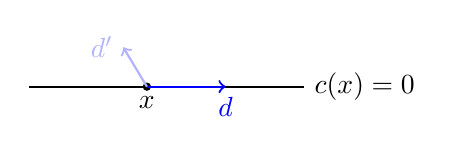
\begin{tikzpicture}[scale=1]
		% Constraint-linje
		\draw[thick] (-1,0) -- (2.5,0) node[right] {$c(x)=0$};
		% Punkt x
		\fill (0.5,0) circle (1.5pt) node[below] {$x$};
		% Tillatt retning
		\draw[->,blue,thick] (0.5,0) -- (1.5,0) node[below] {$d$};
		% Ikke‐tillatt retning
		\draw[->,blue!30,thick] (0.5,0) -- (0.2,0.5) node[left] {$d'$};
	\end{tikzpicture}

	\vspace{0.5ex}
	\small Blå pil: tillatt retning. Lys blå pil: ikke--tillatt retning.
\end{center}

\subsubsection{Tangent kjegle}
En tangentkjegle er en mengde av retninger som vi kan bevege oss i fra et punkt mens vi fortsatt holder oss innenfor mengden \(\Omega\).
Dette er nyttig for å forstå hvilke retninger vi kan utforske når vi søker etter optimale løsninger.

\begin{definition}{Tangentkjegle}{tangent_cone}
	La \(\Omega \subset \R^n\) være en mengde og \(x \in \Omega\) et punkt. Tangentkjeglen er definert som:
	\begin{equation}
		\mathcal{T}_{\Omega}(x) = \left\{ d \in \R^n \;\middle|\; \exists \{z_k\} \subset \Omega, \{t_k\} > 0 : z_k \to x, t_k \to 0, \lim_{k \to \infty} \frac{z_k - x}{t_k} = d \right\}
	\end{equation}
	Den inneholder alle retninger \(d\) som kan oppnås ved å ta små steg innad i mengden \(\Omega\) fra punktet \(x\).
\end{definition}

\begin{center}
	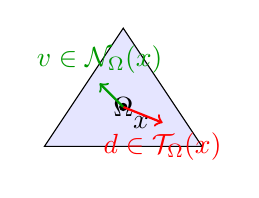
\begin{tikzpicture}[scale=1]
		% Konveks mengde
		\draw[fill=blue!10] (0,0) -- (2,0) -- (1,1.5) -- cycle;
		\node at (1,0.5) {$\Omega$};
		% Punkt x
		\fill (1,0.5) circle (1.5pt) node[below right] {$x$};
		% Tangentretning
		\draw[->,red,thick] (1,0.5) -- (1.5,0.3) node[below] {$d\in\mathcal T_\Omega(x)$};
		% Normalretning
		\draw[->,green!60!black,thick] (1,0.5) -- (0.7,0.8) node[above] {$v\in\mathcal N_\Omega(x)$};
	\end{tikzpicture}

	\vspace{0.5ex}
	\small Rød pil: tangentretning. Grønn pil: normalretning.
\end{center}

Hvis vi velger en retning \(d\) som straks fører oss utenfor de gitte begrensningene \(\Omega\), kan denne retningen utelukkes som mulig løsning.
Det innebærer at når vi vurderer hvilke retninger vi kan søke i, ser vi bort fra de som umiddelbart tar oss utenfor den tillatte mengden \(\Omega\), altså de \(d\) slik at det finnes en \(\varepsilon > 0\) med \(x + t d \notin \Omega\) for alle \(t \in (0, \varepsilon)\).

\subsubsection{Normal kjegle}
\begin{definition}{Normal kjegle}{normal_cone}
	La \(\Omega \subset \R^n\) være en mengde og \(x \in \Omega\) et punkt. Normal kjegle er definert som:
	\[
		\mathcal N_{\Omega}(x) = \Bigl\{d\in\mathbb R^n : d^\top(y - x) \le 0,\;\forall y\in\Omega\Bigr\}
	\]
	Den inneholder alle retninger \(d\) som peker inn i mengden \(\Omega\) fra punktet \(x\).

\end{definition}

\begin{proposition}{Tangentkjegle via Normalkjegle}{tangent_cone_via_normal_cone}
	Tangentkjeglen kan også defineres som den polare konen til normalkjeglen \(\mathcal N_{\Omega}(x)\):
	\[
		\mathcal T_{\Omega}(x)
		=\bigl(\mathcal N_{\Omega}(x)\bigr)^\circ
		=\{d\in\mathbb R^n : v^\top d\le 0,\;\forall\,v\in\mathcal N_{\Omega}(x)\}
	\]
	hvor normalkjeglen er:
	\[
		\mathcal N_{\Omega}(x)
		=\bigl\{v\in\mathbb R^n : v^\top(y - x)\le 0,\;\forall\,y\in\Omega\bigr\}
	\]
\end{proposition}

\subsubsection{Kritisk kjegle}
\begin{definition}{Kritisk kjegle}{critical_cone}
	\(\mathcal C_{\Omega}(x)\) er den kritiske kjeglen til $\Omega$ i punktet $x$.
	Den er definert som
	\[
		\mathcal C_{\Omega}(x)
		=\Bigl\{d\in\mathbb R^n :
		\nabla c_i(x)^\top d = 0,\;i\in\mathcal E,\;
		\nabla c_j(x)^\top d \le 0,\;j\in\mathcal I
		\Bigr\}.
	\]
	Den inneholder alle retninger $d$ som oppfyller de lineære begrensningene i første-ordens og der gradienten $\nabla f(x)$ peker i retningen av $d$.
\end{definition}

\begin{center}
	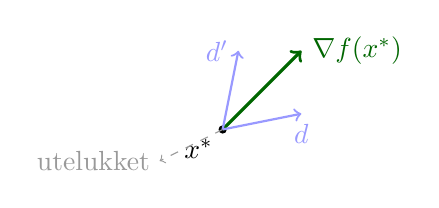
\begin{tikzpicture}[scale=1]
		% Punkt og gradient
		\fill (0,0) circle (1.5pt) node[below left] {$x^*$};
		\draw[->,black!60!green,very thick] (0,0) -- (1,1) node[right] {$\nabla f(x^*)$};
		% Kritiske retninger
		\draw[->,blue!40,thick] (0,0) -- (1,0.2) node[below] {$d$};
		\draw[->,blue!40,thick] (0,0) -- (0.2,1) node[left] {$d'$};
		% Uønsket retning
		\draw[->,gray!80,dashed] (0,0) -- (-0.8,-0.4) node[left] {utelukket};
	\end{tikzpicture}

	\vspace{0.5ex}
	\small Blå piler: kritiske retninger.
	Grå stiplet pil: utelukket retning. Grønn pil: $\nabla f(x^*)$.
\end{center}

\begin{remark}{Inkludering av kjegler}{cone_inclusion}
	For en hvilken som helst mengde \(\Omega\) gjelder følgende inkluderinger:
	\begin{equation}
		\mathcal C_{\Omega}(x) \subseteq \mathcal F_{\Omega}(x) \subseteq \mathcal T_{\Omega}(x)
	\end{equation}
\end{remark}

\begin{proposition}{\(\text{LICQ} \implies \mathcal F_{\Omega}(x) = \mathcal T_{\Omega}(x)\)}{}
	Anta at \(\Omega\) er en konveks mengde og at den lineære uavhengighetsbetingelsen (LICQ) er oppfylt i punktet \(x\). Da er tangentkjeglen lik den linearisert kjeglen:
	\[
		\mathcal F_{\Omega}(x) = \mathcal T_{\Omega}(x)
	\]
\end{proposition}

\section{Funksjoner}

\subsection{Veldefinerte funksjoner}
En funksjon er veldefinert hvis den gir en entydig verdi for hver input--verdi.
\begin{definition}{Veldefinert funksjon}{well_defined}
	La \( f: X \to Y \) være en funksjon. Vi sier at \( f \) er veldefinert hvis:
	\begin{enumerate}
		\item For hvert \( x \in X \) eksisterer det nøyaktig én verdi \( f(x) \in Y \).
		\item Funksjonen er entydig bestemt, det vil si at hvis \( x_1 = x_2 \) så er \( f(x_1) = f(x_2) \).
	\end{enumerate}

	En operator eller en transformasjon er veldefinert hvis den tilfredsstiller de samme kravene: hver innverdi gir nøyaktig én utverdi, og like innverdier gir like utverdier.
\end{definition}

\subsection{Affine funksjoner}
\begin{definition}{Affin funksjon}{affine_function}
	En funksjon $f: \R^n \to \R^m$ er affin hvis den kan skrives på formen:
	\[
		f(\mathbf{x}) = A\mathbf{x} + \mathbf{b}
	\]
	hvor $A \in \R^{m \times n}$ og $\mathbf{b} \in \R^m$.
\end{definition}

\begin{remark}{Egenskaper ved affine funksjoner}{affine_properties}
	\begin{enumerate}
		\item En affin funksjon er summen av en lineær funksjon $L(\mathbf{x}) = A\mathbf{x}$ og en konstant vektor $\mathbf{b}$.
		\item Affine funksjoner bevarer konvekse kombinasjoner:
			  \[
				  f(\lambda \mathbf{x} + (1-\lambda)\mathbf{y}) = \lambda f(\mathbf{x}) + (1-\lambda)f(\mathbf{y}), \quad \forall \lambda \in \R
			  \]
		\item En affin funksjon er både konveks og konkav.
	\end{enumerate}
\end{remark}

\begin{example}{Eksempler på affine funksjoner}{affine_examples}
	\begin{itemize}
		\item $f(x) = 3x + 2$
		\item $f(\mathbf{x}) = \mathbf{c}^T\mathbf{x} + d$ (en lineær funksjon med skalar forskyvning)
		\item $f(x,y) = 2x - 3y + 4$
	\end{itemize}
\end{example}

\subsection{Nedre semi-kontinuerlige funksjoner}
En nedre semikontinuerlig funksjon (\emph{lower semi-continuous function (lsc)}) er en funksjon som ikke har plutselige "hopp nedover".

Tenk deg at du nærmer deg et punkt \( \symbf{x_0} \) fra alle mulige retninger:
\begin{itemize}
	\item Verdien av funksjonen i \( \symbf{x_0} \) vil ikke være høyere enn verdiene du ser når du kommer nærmere.
	\item Funksjonen kan ha "hopp oppover".
\end{itemize}

\begin{definition}{Nedre semi-kontinuerlig funksjoner (LSC)}{lower_semi_continuous}
	\(f: \Omega (\subset \R^d) \to \overline{\R}\) være en funksjon. Vi sier at \(f\) er nedre semi-kontinuerlig (lsc) i punktet \(x_0\) hvis for alle \(\varepsilon > 0\) finnes det en \(\delta > 0\) slik at
	\[
		f(x) > f(x_0) - \varepsilon \quad \text{for alle} \quad x \in B(x_0, \delta).
	\]
	\begin{enumerate}
		\item \(f\) er (lsc) i \(x_0\) hvis det for alle \(\alpha \in \R\) er mengden \(\mathcal{L}_f(\alpha) = \{x | f(x) < \alpha \} \text{ er åpen i } \R^d\)
		\item \(f\) er (lsc) i \(x_0 \in X\) hvis og bare hvis: \(\liminf_{x \to x_0} f(x) \geq f(x_0)\).
	\end{enumerate}
\end{definition}
\begin{example}{Eksempel på en nedre semi-kontinuerlig funksjon}{}
	\begin{figure}[H]
		\centering
		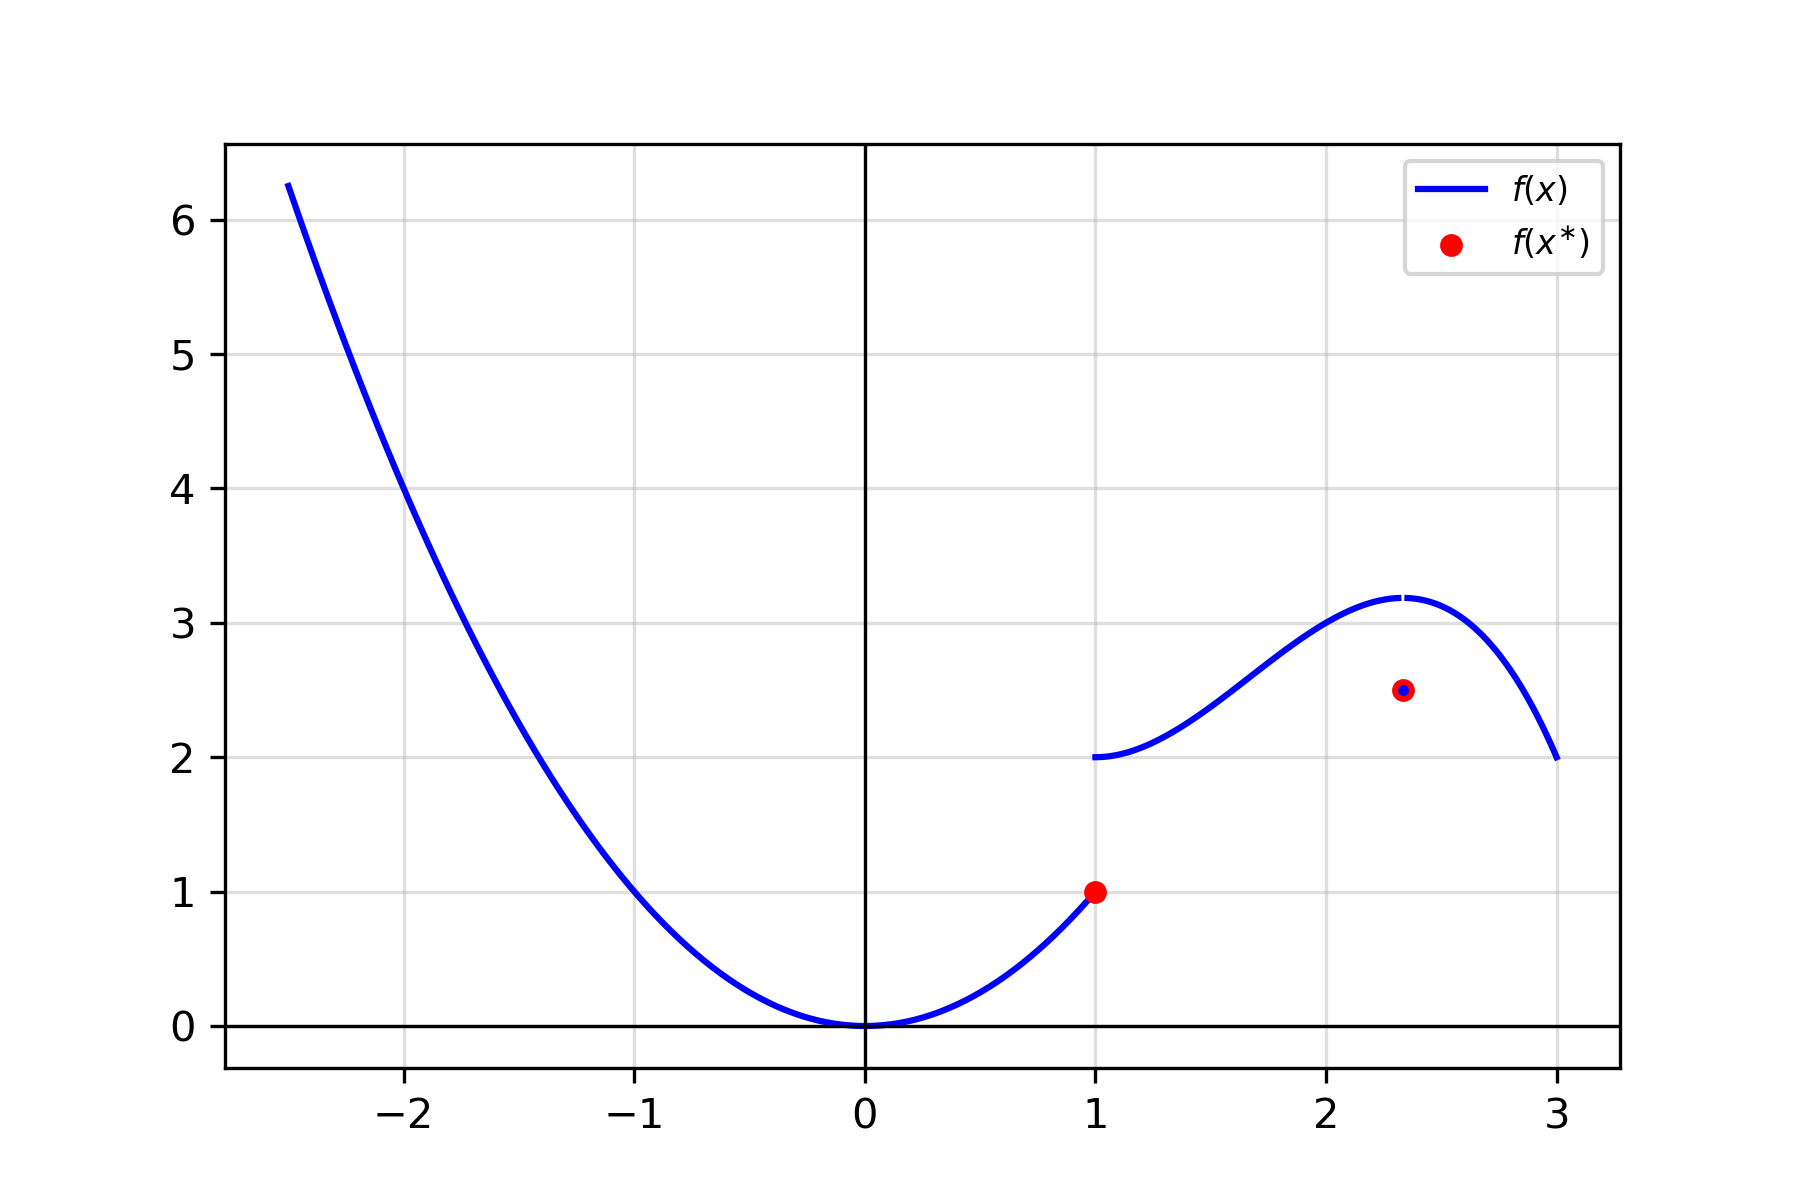
\includegraphics[width=0.5\textwidth]{figures/example_lsc.png}
		\caption{Eksempel på en nedre semi-kontinuerlig funksjon}
	\end{figure}
\end{example}
\begin{remark}{LSC og kontinuerlige funksjoner}{}
	En kontinuerlig funksjon er alltid nedre semi-kontinuer
\end{remark}

\subsection{Koersivitet}
En koersiv funksjon er en funksjon som vokser mot uendelig når vi beveger oss mot kanten av definisjonsmengden.
\begin{definition}{Koersivitet}{coercive}
	En funksjon \(f: \Omega \to \R\) er koersiv hvis for alle \(y \in \R\) er nivåmengden \(\mathcal{L}_f(y) = \{x \in \Omega | f(x) \leq y\}\) kompakt.

	\[
		\lim_{\norm{x} \to +\infty} f(x) = +\infty
	\]
\end{definition}

\subsection{Infimum og Supremum}
\begin{definition}{Infimum}{infimum}
	Infimum (eller nedre grense) av en mengde \(A\) er det største tallet som er mindre enn eller lik alle elementene i \(A\).
	\[
		\inf A = \sup \{x \in \R \mid x \leq a, \forall a \in A\}
	\]
	\begin{itemize}
		\item Hvis \(A\) har et minimum, er infimum lik minimum.
		\item Hvis \(A\) ikke har et minimum, er infimum det største tallet som er mindre enn alle elementene i \(A\).
	\end{itemize}
\end{definition}

Tenk på infimum som den \enquote{laveste støtten} eller \enquote{gulvet} under mengden. Det er den største verdien som fungerer som en nedre grense for alle elementer i mengden. Som et fysisk bilde: hvis elementene i mengden er baller som faller, er infimum den høyeste plattformen som ingen ball kan falle gjennom.

\begin{remark}{Huskeregel}{}
	\enquote{IN-fimum er den største verdien INNenfor eller rett under mengden} (tenk på \enquote{in} som \enquote{inn} eller \enquote{innunder}).
\end{remark}

\begin{example}{Eksempel på infimum}{}
	\begin{itemize}
		\item \(A = \{1, 2, 3\}\) har infimum \(\inf A = 1\).
		\item \(B = \{x \in \R \mid x > 0\}\) har infimum \(\inf B = 0\).
		\item \(C = \{x \in \R \mid x < 0\}\) har infimum \(\inf C = -\infty\).
	\end{itemize}

	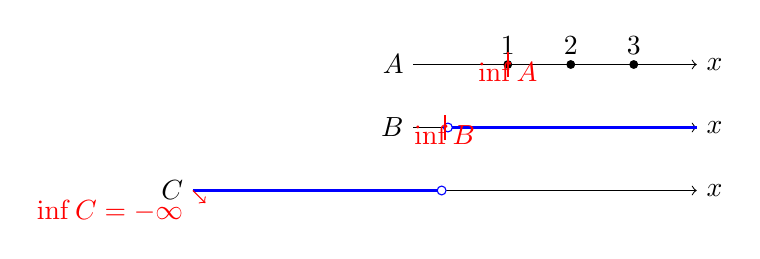
\begin{tikzpicture}[scale=0.8]
		% Example A: discrete set
		\begin{scope}[shift={(0,2)}]
			\draw[->] (-0.5,0) -- (4,0) node[right] {$x$};
			\fill (1,0) circle (2pt) node[above] {1};
			\fill (2,0) circle (2pt) node[above] {2};
			\fill (3,0) circle (2pt) node[above] {3};
			\node[left] at (-0.5,0) {$A$};
			\draw[red,thick] (1,-0.2) -- (1,0.2) node[below] {$\inf A$};
		\end{scope}

		% Example B: x > 0
		\begin{scope}[shift={(0,1)}]
			\draw[->] (-0.5,0) -- (4,0) node[right] {$x$};
			\draw[thick,blue] (0.05,0) -- (4,0);
			\filldraw[blue, fill=white] (0.05,0) circle (2pt);
			\node[left] at (-0.5,0) {$B$};
			\draw[red,thick] (0,-0.2) -- (0,0.2) node[below] {$\inf B$};
		\end{scope}

		% Example C: x < 0
		\begin{scope}[shift={(0,0)}]
			\draw[->] (-4,0) -- (4,0) node[right] {$x$};
			\draw[thick,blue] (-4,0) -- (-0.05,0);
			\filldraw[blue, fill=white] (-0.05,0) circle (2pt);
			\node[left] at (-4,0) {$C$};
			\draw[red,<-] (-3.8,-0.2) -- (-4,0) node[below left] {$\inf C = -\infty$};
		\end{scope}
	\end{tikzpicture}
\end{example}

\begin{definition}{Supremum}{supremum}
	Supremum (eller øvre grense) av en mengde \(A\) er det minste tallet som er større enn eller lik alle elementene i \(A\).
	\[
		\sup A = \inf \{x \in \R \mid x \geq a, \forall a \in A\}
	\]
	\begin{itemize}
		\item Hvis \(A\) har et maksimum, er supremum lik maksimum.
		\item Hvis \(A\) ikke har et maksimum, er supremum det minste tallet som er større enn alle elementene i \(A\).
	\end{itemize}
\end{definition}
Tenk på supremum som \enquote{taket} eller \enquote{den laveste hindringen} over mengden.
Det er den minste verdien som fungerer som en øvre grense for alle elementer i mengden.



\begin{remark}{Supremum huskeregel}{}
	\enquote{SUP-remum er den minste verdien SUpra (over) mengden} (tenk på \enquote{sup} som i \enquote{super} eller \enquote{ovenfor}).
	Som et fysisk bilde: hvis elementene i mengden er hoppende baller, er supremum det laveste taket som ingen ball kan hoppe høyere enn.
\end{remark}

\begin{example}{Eksempel på supremum}{}
	\begin{itemize}
		\item \(A = \{1, 2, 3\}\) har supremum \(\sup A = 3\).
		\item \(B = \{x \in \R \mid x < 0\}\) har supremum \(\sup B = 0\).
		\item \(C = \{x \in \R \mid x > 0\}\) har supremum \(\sup C = +\infty\).
	\end{itemize}

	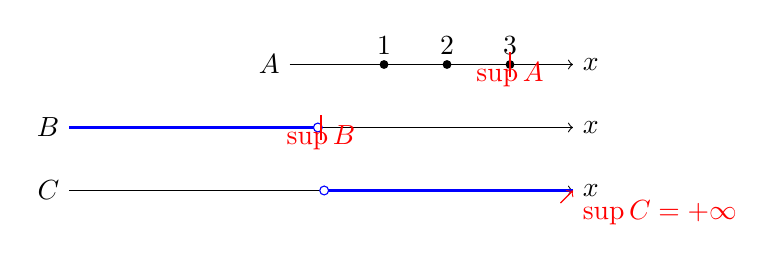
\begin{tikzpicture}[scale=0.8]
		% Example A: discrete set
		\begin{scope}[shift={(0,2)}]
			\draw[->] (-0.5,0) -- (4,0) node[right] {$x$};
			\fill (1,0) circle (2pt) node[above] {1};
			\fill (2,0) circle (2pt) node[above] {2};
			\fill (3,0) circle (2pt) node[above] {3};
			\node[left] at (-0.5,0) {$A$};
			\draw[red,thick] (3,-0.2) -- (3,0.2) node[below] {$\sup A$};
		\end{scope}

		% Example B: x < 0
		\begin{scope}[shift={(0,1)}]
			\draw[->] (-4,0) -- (4,0) node[right] {$x$};
			\draw[thick,blue] (-4,0) -- (-0.05,0);
			\filldraw[blue, fill=white] (-0.05,0) circle (2pt);
			\node[left] at (-4,0) {$B$};
			\draw[red,thick] (0,-0.2) -- (0,0.2) node[below] {$\sup B$};
		\end{scope}

		% Example C: x > 0
		\begin{scope}[shift={(0,0)}]
			\draw[->] (-4,0) -- (4,0) node[right] {$x$};
			\draw[thick,blue] (0.05,0) -- (4,0);
			\filldraw[blue, fill=white] (0.05,0) circle (2pt);
			\node[left] at (-4,0) {$C$};
			\draw[red,->] (3.8,-0.2) -- (4,0) node[below right] {$\sup C = +\infty$};
		\end{scope}
	\end{tikzpicture}
\end{example}

\begin{remark}{Huskeregel for \emph{infimum} og \emph{supremum}}{}
	\textit{INfimum for MINimering, SUPremum for MAKSimering.}
\end{remark}

\subsection{Minimax og maksimin}
Minimax og maksimin er konsepter i optimering som handler om å finne optimale strategier i verst-tenkelige situasjoner.
Minimax beskriver en strategi for å minimere det maksimale potensielle tapet, mens maksimin handler om å maksimere den minimale potensielle gevinsten.

\begin{definition}{Minimax og maksimin}{minimax_maximin}
	For en funksjon $f: X \times Y \to \R$ definerer vi:
	\begin{align*}
		\text{Minimax:}  & \quad \min_{x \in X} \max_{y \in Y} f(x,y) \\
		\text{Maksimin:} & \quad \max_{y \in Y} \min_{x \in X} f(x,y)
	\end{align*}
\end{definition}

\begin{theorem}{Minimax-teoremet}{minimax_theorem}
	La $X$ og $Y$ være kompakte konvekse mengder i $\R^n$, og la $f: X \times Y \to \R$ være kontinuerlig, konveks i $x$ og konkav i $y$. Da har vi:
	\[
		\min_{x \in X} \max_{y \in Y} f(x,y) = \max_{y \in Y} \min_{x \in X} f(x,y)
	\]
\end{theorem}

Dette teoremet er spesielt nyttig i optimering for å analysere verst-tenkelige scenarier og finne robuste løsninger.

\subsection{Konvekse funksjoner}
Konveksitet i matematikk refererer til egenskapene til funksjoner og mengder som har en bestemt form.
I optimering er konveksitet en viktig egenskap fordi den kan fortelle oss om hvordan en funksjon oppfører seg, spesielt når det gjelder å finne minimum eller maksimum verdier.

\begin{itemize}
	\item En konveks funksjon har en bue som vender oppover.
	\item En konkav funksjon har en bue som vender nedover.
	\item En konveks mengde er en mengde der enhver linje mellom to punkter i mengden også ligger helt innenfor mengden.
\end{itemize}

\begin{definition}{Konveks funksjon}{convex_function}
	En funksjon \(f: \R^n \to \R\) er:
	\begin{align*}
		f(\lambda x + (1-\lambda)y) & \leq \lambda f(x) + (1-\lambda)f(y) \quad \forall x, y \in \R^n, \lambda \in [0, 1] \tag{Konveks}                  \\
		f(\lambda x + (1-\lambda)y) & < \lambda f(x) + (1 - \lambda)f(y) \quad \forall x, y \in \R^n, \lambda \in (0, 1), x \neq y \tag{Strengt konveks}
	\end{align*}
\end{definition}

\begin{remark}{Konveksitet med indre-produkt notasjon}{convex_inner_product}
	En funksjon  \(f: \R^n \to \R\) er konveks hvis og bare hvis:
	\[
		f(y) - f(x) \geq  \langle \nabla f(x), y - x \rangle
	\]
	for alle  \(x, y \in \R^n\).
\end{remark}

\begin{remark}{Kvasi--konvekse funksjoner}{quasi_convex_function}
	En funksjon \(f: \R^d \to \R\) er kvasi-konveks hvis for alle \(x, y \in \R^n\) og \(\lambda \in (0, 1)\) har vi:

	\[
		f(\lambda x + (1 - \lambda)y) \leq \max\{f(x), f(y)\}
	\]

	En alternativ definisjon er at en funksjon er kvasi-konveks hvis alle nivåsettene er konvekse.

	\[
		\mathcal{L}_f(y) = \{x \in \R^n | f(x) \leq y\} \quad \text{er konveks for alle} \quad y \in \R
	\]

	\[
		\boxed{\underbrace{\forall \alpha \in \R, \mathcal{L}_f(\alpha) \text{ er konveks}}_{f \text{ er kvasi-konveks }}\Longleftrightarrow \forall x, y \in \R^d,\lambda \text{ s.a. } f(\lambda x + (1-\lambda)y) \leq \max \{ f(x), f(y) \}}
	\]
\end{remark}

\subsection{Taylors teorem}
Taylor-utvikling er en metode for å tilnærme en funksjon ved hjelp av dens deriverte.
Den gir oss en måte å uttrykke funksjonen som en sum av dens verdier og deriverte i et punkt, noe som kan være nyttig for å analysere oppførselen til funksjonen i nærheten av det punktet.

Ved hjelp av Taylor-utvikling kan vi avgjøre om \(\symbf{x}^\star\) er en lokal løsning ved å sjekke om gradienten \(\nabla f(\symbf{x}^\star) = 0\) og Hesse-matrisen \(\nabla^2 f(\symbf{x}^\star)\)

\begin{theorem}{Taylors teorem}{taylors_theorem}
	Anta at \(f: \R^n \to \R\) med \(\mathbf{p}\in\R^n\), og la \(t\in[0,1]\).

	\medskip

	Hvis \(f\in\Ccal^1\) (én gang kontinuerlig deriverbar):
	\[
		f(\mathbf{x} + \mathbf{p}) = f(\mathbf{x}) + \nabla f(\mathbf{x}+t\mathbf{p})^\top \mathbf{p},
	\]

	Hvis \(f \in \Ccal^2\) (to ganger kontinuerlig deriverbar):

	\begin{align*}
		\nabla f(\mathbf{x} + \mathbf{p}) = \nabla f(\mathbf{x}) + \int_0^1 \nabla^2 f(\mathbf{x}+t\mathbf{p})\mathbf{p} dt, \\
		\boxed{f(\mathbf{x} + \mathbf{p}) = f(\mathbf{x}) + \nabla f(\mathbf{x})^\top \mathbf{p} + \frac{1}{2}\mathbf{p}^\top \nabla^2 f(\mathbf{x}+t\mathbf{p})\mathbf{p}}
	\end{align*}
\end{theorem}

\section{Andre Viktige Definisjoner, Teoremer og Ekvivalenser}

\subsection{Simplex}
Et simplex er en geometrisk figur som kan forstås som den enkleste formen i et gitt antall dimensjoner. For eksempel er et 0-simplex et punkt, et 1-simplex er en linje, et 2-simplex er en trekant, og så videre.

\begin{definition}{Simplex}{simplex}
	Et simplex i \( \mathbb{R}^n \) er et \( n \)-dimensjonalt objekt laget av \( n+1 \) punkter (hjørner) som ikke ligger i samme hyperplan.

	\begin{figure}[H]
		\centering
		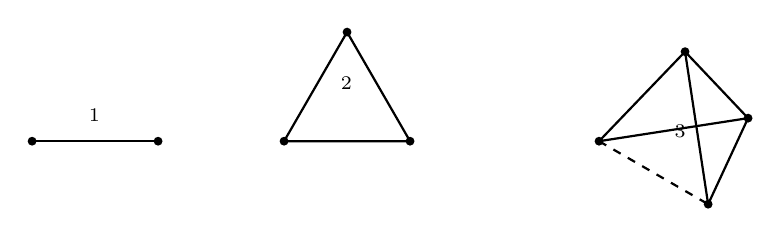
\begin{tikzpicture}[scale=0.8]
			% R1 simplex (line)
			\begin{scope}[shift={(-4,0)}]
				\draw[thick] (0,0) -- (2,0);
				\fill (0,0) circle (2pt);
				\fill (2,0) circle (2pt);
				\node[above] at (1,0) {\( \R^1 \)};
			\end{scope}

			% R2 simplex (triangle)
			\begin{scope}[shift={(0,0)}]
				\draw[thick] (0,0) -- (2,0) -- (1,1.732) -- cycle;
				\fill (0,0) circle (2pt);
				\fill (2,0) circle (2pt);
				\fill (1,1.732) circle (2pt);
				\node[above] at (1,0.5) {\( \R^2 \)};
			\end{scope}

			% R3 simplex (tetrahedron)
			\begin{scope}[shift={(5,0)}, x={(0.866cm,-0.5cm)}, y={(0.866cm,0.5cm)}, z={(0cm,1cm)}]
				% Back triangle
				\draw[thick,dashed] (0,0,0) -- (2,0,0);
				\draw[thick] (2,0,0) -- (1,1.732,0) -- (0,0,0);
				% Vertical edges to top point
				\draw[thick] (0,0,0) -- (1,0.577,1.633);
				\draw[thick] (2,0,0) -- (1,0.577,1.633);
				\draw[thick] (1,1.732,0) -- (1,0.577,1.633);
				% Points
				\fill (0,0,0) circle (2pt);
				\fill (2,0,0) circle (2pt);
				\fill (1,1.732,0) circle (2pt);
				\fill (1,0.577,1.633) circle (2pt);
				\node[above] at (1,0.5,0) {\( \R^3 \)};
			\end{scope}
		\end{tikzpicture}
		\caption{Simplex i ulike dimensjoner.}
	\end{figure}
\end{definition}


\chapter{Optimeringsproblemet}
\label{chap:optimization_problem}

Optimering er et felt innen matematikken som handler om å finne den beste løsningen på et gitt problem, enten med eller uten restriksjoner på løsningsrommet.
Målet i et \emph{optimeringsproblem} er å finne en variabel \(x^\star \in \Omega\) som minimerer eller maksimerer en gitt funksjon \(f: \Omega \to \R\),
kalt \emph{mål\-funksjonen} eller \emph{kostnads\-funksjonen}.

\begin{mini!}{\mathbf{x}}{f(\mathbf{x})}{}{}
\label{eq:opt_problem}
\tag{P}
\addConstraint{\mathbf{x}, \mathbf{x}^\star \in \Omega \subseteq \R^n}
\addConstraint{f: \Omega \to \R}
\addConstraint{f(\mathbf{x}^\star) = \begin{cases}
		\min_{\mathbf{x} \in \Omega} f(\mathbf{x}) & \text{(minimization)} \\
		\max_{\mathbf{x} \in \Omega} f(\mathbf{x}) & \text{(maximization)}
	\end{cases}}
\end{mini!}

\section{Problemformulering}
\label{sec:problem_formulation}
For å forstå optimering, må vi først definere hva et optimeringsproblem er.
I et optimeringsproblem ønsker vi å finne den beste løsningen fra en mengde mulige løsninger, som er definert ved hjelp av en funksjon \(f\) og et søkeområde \(\Omega\).

\subsection{Objektivfunksjon}
Funksjonen \(f\) kalles \emph{mål\-funksjonen} eller \emph{kostnads\-funksjonen}, og den representerer det vi ønsker å minimere eller maksimere.
Funksjonen \(f\) kan være en hvilken som helst funksjon som tar inn en vektor \(x\) fra mengden \(\Omega\) og returnerer et reelt tall.

\subsection{Søkeområde}
Mengden \(\Omega\) betegner de tillatte løsningene og kalles ofte \emph{søkeområdet} eller den \emph{tillatte mengden (eng. feasible set)}.
Ulike typer av søkeområder resulterer i forskjellige typer optimeringsproblemer:
\begin{itemize}
	\item \textbf{Ubetinget optimering:} \(\Omega = \R^n\)
	\item \textbf{Betinget optimering:} \(\Omega \subset \R^n\) er definert ved likninger og/eller ulikheter
	\item \textbf{Konveks optimering:} \(\Omega\) er en konveks mengde
\end{itemize}

\subsection{Optimeringsproblemet}
Dermed kan vi definere et optimeringsproblem som følger:
\begin{definition}{Optimeringsproblemet \((P)\)}{def:optimization_problem}

	La \(f: \Omega \to \R\) være en funksjon vi ønsker å minimere eller maksimere, der \(\Omega \subseteq \R^d\) er mengden av tillatte (mulige) løsninger.
	\[
		\min_{x \in \Omega} f(x) \quad \text{eller} \quad \max_{x \in \Omega} f(x) \tag{P}
	\]
\end{definition}

Vi ønsker som oftest å minimere funksjonen \(f\) over mengden \(\Omega\), og vi kaller dette \emph{minimeringsproblemet}.
Men vi kan like enkelt omformulere problemet til et \emph{maksimeringsproblem} ved å erstatte \(f(x)\) med \(-f(x)\).
De fleste algoritmene og metodene som vi diskuterer, er designet for å løse minimeringsproblemer.

\subsection{Problemklasser}
\label{sec:problem_classes}
Ulike problemtyper oppstår ut fra hvordan denne mengden \(\Omega\) er definert, og hvilke egenskaper funksjonen \(f\) har.

Vi skiller mellom tre hovedtyper av optimeringsproblemer, \emph{ubetinget optimering}, \emph{betinget optimering} og \emph{konveks optimering}.

\subsubsection{Ubetinget Optimering}
Ubetinget optimering er den enkleste typen optimeringsproblemer, hvor man ikke har restriksjoner på variabelen \(\symbf{x}^\star\), hvor vi ønsker å minimere \(f(x)\) over hele rommet \(\R^d\).
\begin{definition}{Ubetinget optimering}{unconstrained_optimization}
\begin{mini!}{\mathbf{x}}{f(\mathbf{x})}{}{}
\label{eq:unconstrained_optimization}
\tag{P}
\addConstraint{\mathbf{x}, \mathbf{x}^\star \in \R^d}
\addConstraint{f: \R^d \to \R}
\addConstraint{f(\mathbf{x}^\star) = \min_{\mathbf{x} \in \R^d} f(\mathbf{x})}
\end{mini!}
\end{definition}

\subsubsection{Betinget Optimering}
Betinget optimering er når vi har restriksjoner på den tillatte mengden \(\Omega \subseteq \R^d\). I motsetning til ubetinget optimering kan vi ikke lenger søke over hele rommet \(\R^d\), men må holde oss innenfor spesifikke begrensninger.
Disse er ofte definert ved hjelp av ulikheter og likheter.
\begin{definition}{Betinget optimering}{constrained_optimization}
\begin{mini!}{\mathbf{x}}{f(\mathbf{x})}{}{}
\label{eq:constrained_optimization}
\tag{P}
\addConstraint{\mathbf{x}, \mathbf{x}^\star \in \Omega \subseteq \R^d}
\addConstraint{f: \Omega \to \R}
\addConstraint{f(\mathbf{x}^\star) = \min_{\mathbf{x} \in \Omega} f(\mathbf{x})}
\end{mini!}
\end{definition}


Da kan vi definere den tillatte mengden \(\Omega\) som:
\begin{definition}{Tillatt mengde}{feasible_set}
	\[
		\Omega = \{ x \in \R^d \mid g_i(x) \leq 0, \, i \in \mathcal{I}, \quad h_j(x) = 0, \, j \in \mathcal{E} \}
	\]
	\begin{itemize}
		\item \textbf{Ulikheter:} \(g_i(x) \leq 0\) for \(i \in \mathcal{I}\)
		\item \textbf{Likheter:} \(h_j(x) = 0\) for \(j \in \mathcal{E}\)
	\end{itemize}
\end{definition}


Under dette igjen kan vi igjen klassifisere 3 bundne optimeringsproblemtyper:
\paragraph{Lineær programmering (LP):} Når \(f\) og restriksjonene er lineære.
\paragraph{Ikke-lineær programmering (NLP):} Når én eller flere av \(f\), \(g_i\), eller \(h_j\) er ikke-lineære.
\paragraph{Kvadratisk programmering (QP):} Når \(f\) er kvadratisk og restriksjonene er lineære.

\subsubsection{Konveks Optimering}
Konveks optimering er en spesialklasse av optimeringsproblemer der både målfunksjonen \(f\) og den tillatte mengden \(\Omega\) er konvekse. Dette betyr at:

\begin{itemize}
	\item \(f\) er en konveks funksjon, dvs. for alle \(x, y \in \Omega\) og \(\lambda \in [0, 1]\):
	      \[
		      f(\lambda x + (1-\lambda)y) \leq \lambda f(x) + (1-\lambda)f(y).
	      \]
	\item \(\Omega\) er en konveks mengde, dvs. for alle \(x, y \in \Omega\) og \(\lambda \in [0, 1]\):
	      \[
		      \lambda x + (1-\lambda)y \in \Omega.
	      \]
\end{itemize}

Konveks optimering er viktig fordi det finnes effektive algoritmer for å løse slike problemer, og enhver lokal løsning er også en global løsning.

\section{Løsninger}
\label{sec:solutions}
I optimeringsproblemer er det viktig å skille mellom globale og lokale løsninger. En global løsning er den beste løsningen i hele søkeområdet, mens en lokal løsning er den beste løsningen i et begrenset område rundt et punkt.\footnote{\(\text{Løsning} = \text{Minimum} = \text{Optimal}\)}

\subsection{Globale løsninger}
En global løsning er den beste løsningen i hele søkeområdet \(\Omega\). Dette betyr at det ikke finnes noen annen løsning i hele \(\Omega\) som gir en bedre verdi for funksjonen \(f\).

\begin{definition}{Globale løsninger}{global_solution}

	\medskip
	For en funksjon \(f: \Omega \to \R\) sier vi at \(\symbf{x}^\star \in \Omega\) er en global løsning av minimeringsproblemet~\eqref{eq:global_minimization_problem} hvis:

	\begin{align*}
		f(\symbf{x}^\star) & \leq f(\symbf{x}) \quad \forall \symbf{x} \in \Omega \tag{Global}                                      \\
		f(\symbf{x}^\star) & < f(\symbf{x}) \quad \forall \symbf{x} \in \Omega, \symbf{x} \neq \symbf{x}^\star \tag{Strengt Global}
	\end{align*}
\end{definition}

\subsubsection{Eksistens av globale løsninger}

En funksjon \(f: \Omega \subset \R^d \to \overline{\R}\) har en global løsning (minimum) i \(\Omega\) hvis den er:

\begin{itemize}
	\item \textbf{Nedre semi-kontinuerlig}: For alle \(x \in \Omega\) og alle sekvenser \((x_n)\) som konvergerer mot \(x\):
	      \[
		      f(x) \leq \liminf_{n \to \infty} f(x_n).
	      \]
	\item \textbf{Koersiv}: Det finnes en konstant \(M > 0\) slik at
	      \[
		      f(x) \geq M \quad \forall x \in \Omega.
	      \]
	      Dette sikrer at \(f\) ikke går mot \(-\infty\) når \(x\) går mot uendelig.
\end{itemize}

\begin{theorem}{Eksistens av globale løsninger}{existence_of_global_solution}
	La \(f: \Omega \subset \R^d \to \overline{\R}\) være nedre semi-kontinuerlig og koersiv på \(\Omega\). Da har \(f\) en global løsning (minimum) i \(\Omega\).
\end{theorem}

\subsection{Lokale løsninger}
En lokal løsning er den beste løsningen i et begrenset område rundt et punkt \(\symbf{x}^\star\).
For å avgjøre om \(\symbf{x}^\star\) er en lokal løsning, må vi undersøke om det finnes bedre løsninger i nærheten.
De fleste metoder for dette baseres på Taylor-utvikling \ref{thm:taylors_theorem}.


\begin{definition}{Lokal løsning}{}
	La \(f: \Omega \to \R\) være en funksjon.

	Vi sier at \(x^\star \in \Omega\) er en lokal løsning av optimeringsproblemet hvis, for en viss \(\varepsilon > 0\):

	\begin{align*}
		f(\symbf{x}^\star) & \leq f(\symbf{x}) \quad \forall \; \symbf{x} \in B(\symbf{x}^\star, \varepsilon) \cap \Omega,                                                  \\
		f(\symbf{x}^\star) & < f(\symbf{x}) \quad \forall \; \symbf{x} \in B(\symbf{x}^\star, \varepsilon) \cap \Omega, \symbf{x} \neq \symbf{x}^\star. \tag{Strengt lokal}
	\end{align*}

	hvor \(B(\symbf{x}^\star, \varepsilon)\) er en åpen kule med sentrum \(\symbf{x}^\star\) og radius \(\varepsilon\)~\ref{def:open_ball}.
\end{definition}

\subsection{Isolerte lokale løsninger}
En isolert lokal løsning er en lokal løsning der det ikke finnes andre løsninger i nærheten. Dette betyr at det er en viss avstand fra \(\symbf{x}^\star\) til alle andre løsninger.

\begin{lemma}{Isolert lokal løsning}{isolated_local_solution}
	La \(f: \Omega \to \R\) være en funksjon.

	Hvis \(\symbf{x}^\star \in \Omega\) er en isolert lokal løsning, finnes det en \(\varepsilon > 0\) slik at:

	\[
		f(\symbf{x}^\star) \leq f(\symbf{x}) \quad \forall \; \symbf{x} \in B(\symbf{x}^\star, \varepsilon) \cap \Omega, \symbf{x} \neq \symbf{x}^\star.
	\]
\end{lemma}

\section{Optimalitetsbetingelser}

\subsection{Første Ordens Nødvendige Betingelser}

For en lokal løsning \(\mathbf{x}^\star\) må gradienten være null:

\begin{theorem}{First-Order Necessary Conditions}{first_order_necessary_conditions}
	Hvis \(\mathbf{x}^\star\) er et lokalt minimum, og \(f\) er kontinuerlig deriverbar rundt \(\mathbf{x}^\star\), da er:
	\[
		\nabla f(\mathbf{x}^\star) = 0.
	\]
\end{theorem}

\subsubsection{Stasjonære punkter}
Stasjonære punkter er punkter der gradienten til funksjonen er null. Dette betyr at det ikke er noen retning der funksjonen øker eller minker, og det kan være et minimum, maksimum eller et sadelpunkt.

\begin{corollary}{Stasjonære punkter}{stationary_points}
	La \(f: \Omega \to \R\) være en funksjon. Et punkt \(\symbf{x}^\star \in \Omega\) er et stasjonært punkt hvis:
	\[
		\nabla f(\symbf{x}^\star) = 0.
	\]
	Dette betyr at gradienten til \(f\) i punktet \(\symbf{x}^\star\) er lik null.
\end{corollary}

\subsubsection{Konvergens mot stasjonære punkter}
Når vi bruker iterative metoder for å finne minimum av en funksjon \(f\), ønsker vi å vite om algoritmen vil konvergere til det stasjonære punktet \(\symbf{x}^\star\).

\begin{theorem}{Konvergens til stasjonære punkter}{convergence_to_stationary_points}
	Anta at \(f: \R^d \to \R\) er en kontinuerlig deriverbar funksjon, og at følgende betingelser er oppfylt:
	\begin{enumerate}
		\item \(\Omega\) er en lukket og begrenset mengde.
		\item \(f(\symbf{x})\) er koersiv.
		\item \(f(\symbf{x})\) er nedre semi-kontinuerlig.
		\item \(\nabla f(\symbf{x})\) eksisterer og er Lipschitz-kontinuerlig.
		\item \(\nabla^2 f(\symbf{x})\) eksisterer og er Lipschitz-kontinuerlig.
	\end{enumerate}
	Da konvergerer sekvensen \((\symbf{x}_k)\) generert av en optimaliseringsalgoritme til et stasjonært punkt \(\symbf{x}^\star\) i \(\Omega\).
	\[
		\lim_{k \to \infty} \|\nabla f(\symbf{x}_k)\| = 0.
	\]

	hvor \(\symbf{x}_k\) er iteratene generert av en optimaliseringsalgoritme, og \(\symbf{x}^\star\) tilfredsstiller de førsteordens nødvendige betingelsene \(\nabla f(\symbf{x}^\star) = 0\).

\end{theorem}

\subsection{Andre Ordens Nødvendige Betingelser}

For en lokal løsning må både gradienten være null og Hesse-matrisen positiv definit:

\begin{theorem}{Second-Order Necessary Conditions}{second_order_necessary_conditions}
	Hvis \(\mathbf{x}^\star\) er et lokalt minimum, og \(f\) er to ganger kontinuerlig deriverbar rundt \(\mathbf{x}^\star\), da er:
	\[
		\nabla f(\mathbf{x}^\star) = 0 \quad \text{og} \quad \nabla^2 f(\mathbf{x}^\star) \succeq 0.
	\]
\end{theorem}

\subsection{Andre Ordens Tilstrekkelige Betingelser}

\begin{theorem}{Second-Order Sufficient Conditions}{second_order_sufficient_conditions}
	Hvis \(\nabla f(\mathbf{x}^\star) = 0\) og \(\nabla^2 f(\mathbf{x}^\star) \succ 0\) (positiv definit), da er \(\mathbf{x}^\star\) et \emph{strengt lokalt minimum}.

	\medskip

	Det vil si at det finnes en \(\varepsilon > 0\) slik at:
	\[
		f(\mathbf{x}^\star) < f(\mathbf{x})  \quad \forall \; \mathbf{x} \in B(\mathbf{x}^\star, \varepsilon) \cap \Omega, \mathbf{x} \neq \mathbf{x}^\star.
	\]
\end{theorem}

\section{Optimalitet og konveksitet}
\label{sec:optimality_and_convexity}
For en konveks funksjon \(f\) er det stasjonære punktet \(\mathbf{x}^\star\) også et globalt minimum. Dette er en viktig egenskap ved konvekse funksjoner, og det gjør dem spesielt nyttige i optimering.

\begin{remark}{Konveksitet og stasjonære punkter}{convexity_and_stationary_points}
	\begin{itemize}
		\item Hvis \(f\) er \textbf{konveks} så er alle lokale minimum \(\mathbf{x}^\star\) også globale minimum.
		\item Hvis \(f\) er \textbf{konveks} og \textbf{deriverbar} så er alle stasjonære punkter \(\mathbf{x}^\star\) også globale minimum.
	\end{itemize}
\end{remark}

\begin{example}{Eksistens og optimalitet}{}
	For \( f(x) = x^2 + 2x \), som er kontinuerlig og koersiv, finnes et globalt minimum i \( x^* = -1 \) der \( f(-1) = -1 \).
\end{example}
\begin{example}{Eksistens og optimalitet}{}
	For \( f(x) = x^2 \), har vi \( \nabla f(x) = 2x \). I \( x^* = 0 \) er \( \nabla f(0) = 0 \) og \( \nabla^2 f(x) = 2 > 0 \), som oppfyller SOSC.
\end{example}

